\chapter{Stabilit\`a e funzioni di Lyapunov}
In questo capitolo e nel prossimo andiamo a studiare come si comportano i punti fissi\footnote{in questo studiamo la stabilit\`a, nel prossimo cercheremo quando possibile di descrive un comportamento pi\`u preciso}. Raccolte queste informazioni sui punti stabili speriamo di poterle poi ``incollare" per raggiungere un'idea sufficientemente accurata del comportamento dell'intero sistema.

\section{Stabilit\`a per Lyapunov}
\begin{definition}[Punti stabili per Lyapunov]
Un punto $x\in\R^d$ si dice 
\setlength{\leftmargini}{0.3cm}
\begin{itemize}
\item \textbf{stabile} (nel senso di Lyapunov) se per ogni $\e>0$ esiste $\delta>0$ tale che per ogni $y\in B_\delta(x)$ si ha che per ogni $t\geq 0$ abbiamo $\phi_t(y)\in B_\e(\phi_t(x))$.
\item \textbf{asintoticamente stabile} (nel senso di Lyapunov) se \`e stabile (nel senso di Lyapunov) ed esiste un intorno $U$ di $x$ tale che per ogni $y\in U$
\[\lim_{t\to+\infty}d(\phi_t(x),\phi_t(y))=0.\]
\item \textbf{instabile} (nel senso di Lyapunov) se non \`e stabile.
\end{itemize}
\setlength{\leftmargini}{0.5cm}
\end{definition}

\begin{remark}[Stabilit\`a per punti fissi]
Se $x$ \`e un punto fisso \`e stabile nel senso di Lyapunov se per ogni $\e>0$ esiste un $\delta>0$ tale che $d(y,x)<\delta\implies d(\phi_t(y),x)<\e$ per ogni $t\geq 0$. Similmente \`e asintoticamente stabile nel senso di Lyapunov se \`e stabile ed esiste un intorno $U$ tale che $\forall y\in U$ abbiamo $\displaystyle\lim_{t\to+\infty}\phi_t(y)= x$.
\end{remark}

\begin{definition}[Stabilit\`a orbitale]
Un insieme\footnote{preferibilmente positivamente invariante} $\Gamma\subseteq \R^d$ \`e \textbf{orbitalmente stabile} se per ogni $\e>0$ esiste $\delta>0$ tale che $d(y,\Gamma)<\delta\implies d(\phi_t(y),\Gamma)<\e$ per ogni $t\geq 0$.
\end{definition}

\begin{definition}[Dominio di asintotica stabilit\`a]
Se $x_0$ \`e un punto asintoticamente stabile definiamo il \textbf{dominio di asintotica stabilit\`a} come
\[\cpa{y\in\R^d\mid \omega(y)=\cpa{x_0}}.\]
\end{definition}

\begin{remark}[Convergenza non \`e sufficiente per asintotica stabilit\`a]
Esistono punti che rispettano la condizione di convergenza nella definizione di asintotica stabilit\`a che NON sono stabili (e quindi non vengono classificati come asintoticamente stabili).\\
Un punto di questo tipo \`e $(1,0)$ nel sistema (espresso in coordinate polari)
\[\begin{cases}
\dot\rho=\rho(1-\rho^2)\\
\dot\theta=2\sin^2\pa{\frac12\theta}
\end{cases}\]
\begin{figure}[!htb]
    \centering
    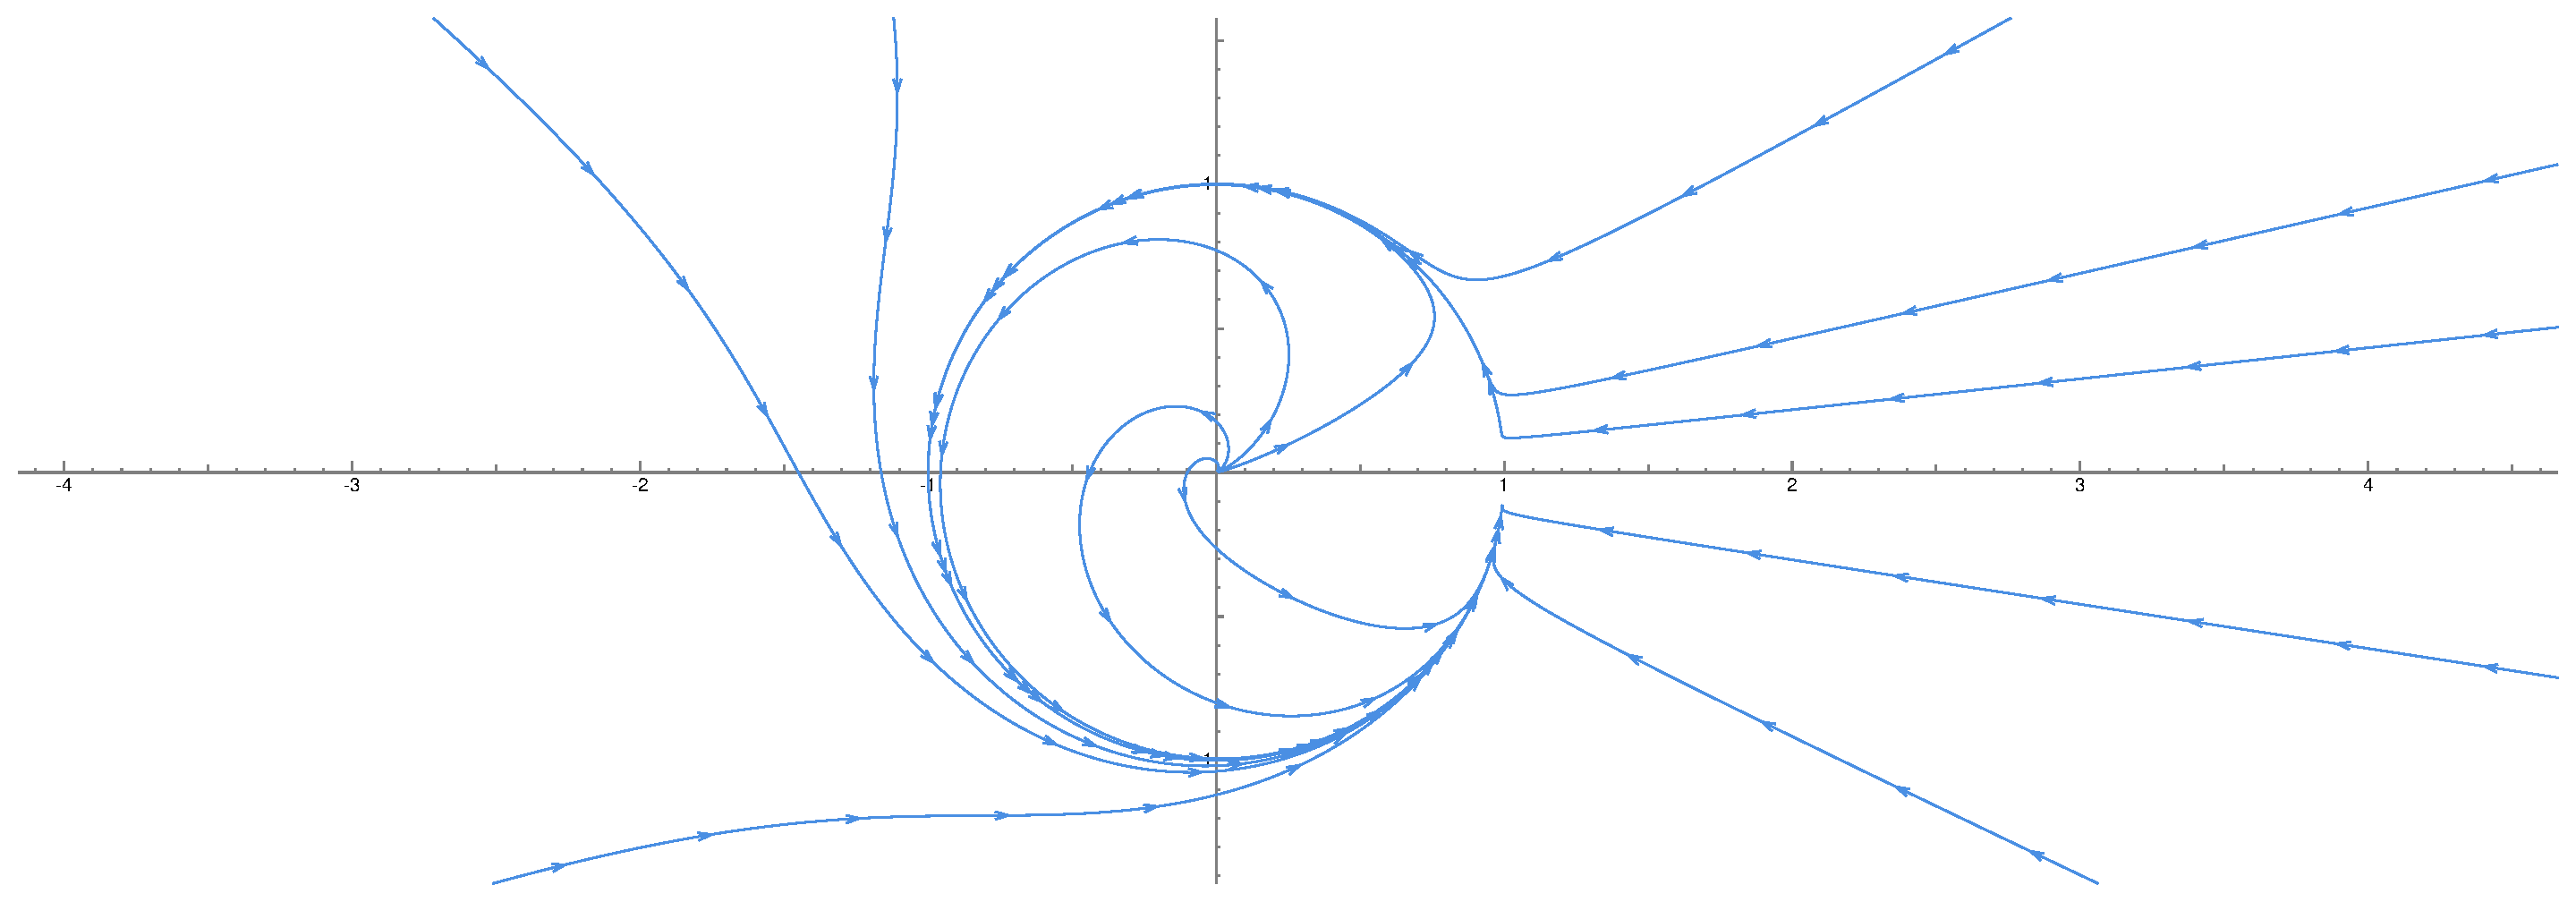
\includegraphics[width=11cm]{Immagini/convergenza_non_asintoticamente_stabile.pdf}
    \caption{In un intorno di $(1,0)$ ci sono sempre punti con $y>0$ e questi ``fanno un giro" prima di convergere.}
\end{figure}
\end{remark}

\section{Funzioni di Lyapunov}
\begin{definition}[Funzione di Lyapunov]
Sia $x_0\in\R^d$ punto fisso per $F\in C^1$ e $U(x_0)$ un suo intorno. Una funzione $V:U(x_0)\to\R$ si dice \textbf{funzione di Lyapunov per $x_0$} se $V\in C^1(U(x_0))$ e
\setlength{\leftmargini}{0.5cm}
\begin{itemize}
\item $V(x)>V(x_0)$ per ogni $x\in U(x_0)\bs \cpa{x_0}$
\item $\dot V(x)=\nabla V(x)\cdot F(x)\leq 0$ per ogni $x\in U(x_0)$.
\end{itemize}
Una funzione di Lyapunov \`e \textbf{stretta} se $\dot V(x)<0$ per ogni $x\in U(x_0)\bs \cpa{x_0}$.
\end{definition}

\begin{theorem}[Primo teorema di Lyapunov]\label{TeoremaLyapunov1Stabilita}
Sia $x_0\in\R^d$ un punto fisso per $F\in C^1$ e $V:U(x_0)\to\R$ una funzione di Lyapunov per $x_0$. Allora $x_0$ \`e un punto stabile nel senso di Lyapunov.
\end{theorem}
\begin{proof}
Fissiamo $\e>0$ tale che $\ol{B_\e(x_0)}\subseteq U(x_0)$. Definiamo \[m=\min_{\del B_\e(x_0)}V,\quad S_m=\cpa{y\in\ol{B_\e(x_0)}\mid V(y)< m}.\]
Osserviamo che $x_0\in S_m$ e, poich\'e $S_m=V\ii((-\infty,m))\cap B_\e(x_0)$, $S_m$ \`e aperto, dunque esiste $\delta>0$ tale che $B_\delta(x_0)\subseteq S_m$.\\
Sia ora $y\in B_\delta(x_0)$. Per definizione $V(y)< m$. Osserviamo che
\[\dd t{}V(\phi_t(y))=\dot V(\phi_t(y))\leq 0 \quad \forall t\geq 0\ t.c.\ \forall 0\leq s\leq t\ \phi_s(y)\in U(x_0),\]
in particolare, per gli stessi valori di $t$, $\phi_t(y)< m$ .\\
Per assurdo supponiamo che esista $\ol t>0$ tale che $\phi_{\ol t}(y)\notin B_\e(x_0)$. Per continuit\`a di $\phi_\cdot(y)$ possiamo supporre $\phi_{\ol t}(y)\in \del B_\e(x_0)$ e tale che per ogni $0\leq s\leq t$ si ha $\phi_s(y)\in U(x_0)$. Si ha dunque $V(\phi_{\ol t}(y))\geq m>V(\phi_t(y))$ per ogni $t\geq 0$ tale che $0\leq s\leq t$ abbiamo $\phi_s(y)\in U(x_0)$, ma $\del B_\e(x_0)\subset\ol B_\e(x_0)\subseteq U(x_0)$, da cui un assurdo.
\end{proof}

\noindent Introduciamo ora un criterio che \`e spesso utile per mostrare l'asintotica stabilit\`a:
\begin{proposition}[Criterio di La Salle]\label{CriterioLaSalle}
Sia $x_0$ un punto fisso per $F\in C^1$ e $V$ una funzione di Lyapunov per $x_0$ su $U(x_0)$. Se $y\in U(x_0)$ \`e tale che $\Oc^+(y)$ \`e limitata e contenuta in $U(x_0)$ allora $\omega(y)$ \`e un insieme non vuoto, compatto e invariante tale che $\omega(y)\subseteq \cpa{\dot V=0}$.
\end{proposition}
\begin{proof}
Se per $y$ valgono le ipotesi, per il criterio di invarianza per $\omega$-limiti (\ref{OrbitaPositivaLimitataImplicaCompattezzaEInvarianzaOmegaLimite}) abbiamo che $\omega(y)$ \`e non vuoto, compatto e invariante.\\
Osserviamo ora che $t\mapsto V(\phi_t(y))$ \`e non crescente e monotona, dunque esiste $\displaystyle c=\lim_{t\to+\infty}V(\phi_t(y))$. Osserviamo ora che
\begin{align*}
z\in \omega(y)&\coimplies \exists t_k\nearrow +\infty \ t.c.\ \phi_{t_k}(y)\to z\implies\\
&\implies V(z)=V\pa{\lim_{k}\phi_{t_k}(y)}\pasgnl={V\text{ cont.}}=\lim_k V(\phi_{t_k}(y))=c.
\end{align*}
Si ha dunque che $\omega(y)\subseteq \cpa{V=c}$. Per l'invarainza di $\omega(y)$ si ha che $V\circ \phi_\cdot(z)\res{\omega(y)}$ \`e costante per ogni $z\in\omega(y)$. Questo significa che $\dot V\res{\omega(y)}=0$, da cui $\omega(y)\subseteq \cpa{\dot V=0}$.
\end{proof}

\begin{remark}
Nelle ipotesi della proposizione, $x_0$ \`e stabile e quindi esiste un $y$ che rispetta le ipotesi.
\end{remark}

\begin{theorem}[Secondo teorema di Lyapunov]\label{TeoremaLyapunov2AsintoticaStabilita}
Sia $x_0\in \R^d$ un punto fisso per $F\in C^1$ e $V:U(x_0)\to\R$ una funzione di Lyapunov stretta per $x_0$, allora $x_0$ \`e asintoticamente stabile.
\end{theorem}
\begin{proof}
Per il primo teorema (\ref{TeoremaLyapunov1Stabilita}) abbiamo che $x_0$ \`e stabile, quindi dobbiamo solo verificare la convergenza.\\
Scelto $\e>0$ sia $\delta>0$ tale che $y\in B_\delta(x_0)$ e $\phi_t(y)\in B_\e(x_0)\subseteq U(x_0)$. Allora per La Salle (\ref{CriterioLaSalle}) $\omega(y)\subseteq \cpa{\dot V=0}\cap U(x_0)=\cpa{x_0}$.
\end{proof}

\begin{remark}
Se $V:U(x_0)\to\R$ \`e una funzione di Lyapunov stretta per $x_0$ allora
\[V_m=\cpa{y\in U(x_0)\mid V(y)\leq m}\]
\`e contenuto nel dominio di asintotica stabilit\`a per ogni $m$ tale che $V_{m}\subseteq U(x_0)$. In particolare vale per $V_{\wt m}$ dove
\[\wt m=\max\cpa{m\mid V_{m}\subseteq U(x_0)}.\]
\end{remark}

\begin{remark}
Se $x_0$ \`e un punto fisso
\setlength{\leftmargini}{0.5cm}
\begin{itemize}
\item Funzione di Lyapunov $\implies$ $x_0$ stabile
\item Funzione di Lyapunov stretta $\implies$ $x_0$ asintoticamente stabile
\item Funzione di Lyapunov + unico insieme invariante di $\cpa{\dot V=0}$ \`e il punto garantiscono comunque asintotica stabilit\`a (per il criterio di La Salle (\ref{CriterioLaSalle}))
\item Se $V:U(x_0)\to \R,\ V\in C^1(U(x_0))$ tale che $V(x)>V(x_0)$ per ogni $x\in U(x_0)\bs\cpa{x_0}$ e $\dot V(x)>0$ per ogni $x\in U(x_0)\bs\cpa{x_0}$ allora $x_0$ \`e \textit{instabile}.
\end{itemize}
\end{remark}

\subsection{Primo approccio per cercare funzioni di Lyapunov}
Nella risoluzione di esercizi spesso si vuole trovare una funzione di Lyapunov. Se non ci sono migliori metodi a disposizione per lo studio del punto, una scelta che di solito funziona quando pu\`o almeno localmente (per $y_0=(y_1,\cdots, y_d)$ punto fisso in esame) \`e
\[V(x_1,\cdots, x_d)=\sum_{i=1}^d a_i (x_i-y_i)^{2n_i},\]
cio\`e costruiamo un paraboloide sopra il punto fisso in esame. Gli insiemi di livello di questa funzione sono paraboloidi contenenti $y_0$.